\documentclass[a4paper,german]{article}
%Mainly taken from
%https://github.com/gillescastel/university-setup/blob/master/preamble.tex
%but edited for own purposes

%%%%%OWN
%%Own basic packages
\usepackage{mkessler-math}
\usepackage{mkessler-fancythm}
\usepackage{mkessler-operators}

\usepackage{datetime}
\date{{\normalfont Mitschrift}\\{\sc Maximilian Keßler} \\ {\small Version} \\ {\small \today\; \currenttime}}

%%%%%%Preamble from Gilles Castel
% Some basic packages
\usepackage{url}
\usepackage{graphicx}
\usepackage{float}

% for wrapping text around figures
\usepackage{wrapfig}

%%This option is for now commented out, not sure what it does, but causes errors
%\pdfminorversion=7


% Don't indent paragraphs, leave some space between them
\usepackage{parskip}

% Hide page number when page is empty
\usepackage{emptypage}
% Other font I sometimes use.
\usepackage{xcolor}
% \usepackage{cmbright}

% Math stuff
\usepackage{amsfonts}

% Put x \to \infty below \lim
\let\svlim\lim\def\lim{\svlim\limits}

%Make implies and impliedby shorter
\let\implies\Rightarrow
\let\impliedby\Leftarrow
\let\iff\Leftrightarrow
\let\epsilon\varepsilon

% Command for short corrections
% Usage: 1+1=\correct{3}{2}

% Environments
\makeatother

% Fix some spacing
% http://tex.stackexchange.com/questions/22119/how-can-i-change-the-spacing-before-theorems-with-amsthm
\makeatletter
\def\thm@space@setup{%
  \thm@preskip=\parskip \thm@postskip=0pt
}


% \lecture starts a new lecture (les in dutch)
%
% Usage:
% \lecture{1}{di 12 feb 2019 16:00}{Inleiding}
%
% This adds a section heading with the number / title of the lecture and a
% margin paragraph with the date.

% I use \dateparts here to hide the year (2019). This way, I can easily parse
% the date of each lecture unambiguously while still having a human-friendly
% short format printed to the pdf.

\usepackage{xifthen}
\def\testdateparts#1{\dateparts#1\relax}
\def\dateparts#1 #2 #3 #4 #5\relax{
    \marginpar{\small\textsf{\mbox{#1 #2 #3 #5}}}
}

\def\@lecture{}%
\newcommand{\lecture}[3]{
    \ifthenelse{\isempty{#3}}{%
    \def\@lecture{\ifenglish Lecture\else Vorlesung\fi\, #1}%
    }{%
\def\@lecture{\ifenglish Lecture\else Vorlesung\fi\, #1: #3}%
    }%
    \subsection*{\@lecture}
    \marginpar{\small\textsf{\mbox{#2}}}
}

% These are the fancy headers
\usepackage{fancyhdr}
\pagestyle{fancy}

% LE: left even
% RO: right odd
% CE, CO: center even, center odd
% My name for when I print my lecture notes to use for an open book exam.
% \fancyhead[LE,RO]{Gilles Castel}

\fancyhead[RO,LE]{\@lecture} % Right odd,  Left even
\fancyhead[RE,LO]{}          % Right even, Left odd

\fancyfoot[RO,LE]{\thepage}  % Right odd,  Left even
\fancyfoot[RE,LO]{}          % Right even, Left odd
\fancyfoot[C]{\leftmark}     % Center

\makeatother

% Todonotes and inline notes in fancy boxes
\usepackage{todonotes}

% Make boxes breakable
\tcbuselibrary{breakable}

% Figure support as explained in my blog post.
\usepackage{import}
\usepackage{xifthen}
\usepackage{pdfpages}
\usepackage{transparent}
\newcommand{\incfig}[1]{%
    \def\svgwidth{\columnwidth}
    \import{./figures/}{#1.pdf_tex}
}

% Fix some stuff
% %http://tex.stackexchange.com/questions/76273/multiple-pdfs-with-page-group-included-in-a-single-page-warning
\pdfsuppresswarningpagegroup=1







\title{{Einführung in die} \\ Geometrie und Topologie}
\author{{\normalfont Dozent}\\{\sc Dr. Daniel Kasprowski}}



\begin{document}
    \maketitle
    \vspace{3em}
    \centering \small Version \\
    \today\; \currenttime
    \vspace{10em}
    \abstract{Bei folgenden Vorlesungsnotizen handelt es sich um (inoffizielle) Mitschriften zur Vorlesung 'Algorithmische Mathematik II', die im Sommersemester 2021 an der Universität Bonn gehalten wird. Ich garantiere weder für Korrektheit noch Vollständigkeit dieser Notizen, und bin dankbar für jegliche Art von Korrektur, sowohl inhaltlich, als auch Tippfehler. \\
Bemerkungen, die nicht zum eigentlichen Vorlesungsinhalte gehören, wurden mit einem * gekennzeichnet. Sie werden nach eigenem Ermessen hinzugefügt, um weitere Details oder evtl. mündliche Anmerkungen beizufügen. \\
Manche Umgebungen sind mit einem $^{\dagger}$ versehen. Das ist dann der Fall, wenn ihr Inhalt so, oder zumindest in sehr ähnlicher Form, in der Vorlesung vorkam (unter Umständen auch mündlich), ich aber die Umgebung der Aussage geändert habe. Das ist z.B. dann der Fall, wenn ich aus Aussagen, die einfach erwähnt werden, ein \textbf{Lemma$^{\dagger}$} mache, um sie hervorzuheben. \\
Weitere Informationen finden sich bei \href{https://github.com/kesslermaximilian/LectureNotesBonn}{GitHub} oder auf der \href{https://wt.iam.uni-bonn.de/ferrari/teaching/lectures-homepages/almaiiss19-1}{Vorlesungshomepage}

    \newpage
    \tableofcontents
    \newpage
    \listoflecture
    \addcontentsline{toc}{section}{Übersicht der Vorlesungen}
    \newpage
    % start lectures
    %! TEX root = ./master.tex
\lecture[Zusammenhang, Wegzusammenhang. Bilder (weg-) zusammenhängender Räume. Lemma von Urysohn.]{Di 11 Mai 2021 12:16}{Zusammenhang}

\section{Zusammenhang, Wegzusammenhang}

\begin{definition}[Zusammenhang]\label{def:zusammenhang}
    Ein topologischer Raum heißt \vocab[Topologischer Raum!zusammenhängend]{zusammenhängend}, wenn er sich \underline{nicht} in zwei nichtleere, disjunkte, offene Teilmengen zerlegen lässt. 
\end{definition}

\begin{dlemma}[Offen-abgeschlossene-Mengen]\label{lm:raum-ist-zusammenhängend-gdw-offen-abgeschlossene-mengen-sind-trivial}
    Ein Raum ist zusammenhängend, wenn die leere Menge und der gesamte Raum die einzigen Teilmengen von $X$ sind, die offen und abgeschlossen sind, d.h.
     \[
    \not \exists  A\subset X, A\neq \emptyset,X \colon \quad A \text{ offen und abgeschlossen}
    .\] 
\end{dlemma}

\begin{proof*}
    Gibt es eine offene, abgeschlossene Menge $A\neq \emptyset,X$, so ist $X = A \sqcup A^{c}$ eine Zerlegung in offene, diesjunkte Mengen. Ist umgekehrt $X = U_1 \cup U_2$ mit $U_1,U_2$ offen, disjunkt und nichtleer, also auch nicht $X$, so sind $U_1,U_2$ beides offen abgeschlossene Mengen.
\end{proof*}

\begin{remark}
    $X$ ist nicht zusammenhängend, genau dann, wenn  $X \cong X_1 \coprod X_2$ eine disjunkte Vereinigung von 2 Räumen $X_1,X_2\neq \emptyset$ ist.
\end{remark}

\begin{example}
    \begin{enumerate}[1)]
        \item $\R\setminus \left \{0\right\}  = (-\infty,0) \cup (0,\infty)$ und $(-\infty,0),(0,\infty)$ sind offen, disjunkt und nicht leer, also ist $\R\setminus \left \{0\right\} $ \underline{nicht} zusammenhängend. 
        \item Betrachte $\Q\subset \R$ mit der Unterraumtopologie. Dann ist
            \[
                \Q = (\Q \cap (-\infty,\sqrt{2})) \cup (\Q \cap (\sqrt{2},\infty))  
            .\] 
            eine Zerlegung in offene, disjunkte, nichtleere Mengen, also ist auch $\Q$ nicht zusammenhängend.
    \end{enumerate}
\end{example}

\begin{remark*}
    Es ist meistens einfacher, zu zeigen, dass ein Raum nicht zusammenhängend ist, die Gegenrichtung erweist sich als schwerer. Deswegen folgender
\end{remark*}

\begin{theorem}[Einheitsintervall]\label{thm:einheitsintervall-ist-zusammenhängend}
    Das Intervall $[0,1]$ ist zusammenhängend.
\end{theorem}

\begin{proof}
    Nimm gegenteilig an, dass $[0,1]$ nicht zusammenhängend ist, schreibe also  $[0,1] = A \cup B$ mit $A,B \neq \emptyset$, offen und disjunkt. OBdA sei $0\in A$. Wegen $B\neq \emptyset$ gibt es $t:= \inf B$. Da  $t$ abgeschlossen (weil  $A$ offen!), ist  $t\in B$, also folgt $[0,t) \subset A$. Aber jede Umgebung von $t\in B$ schneidet $[0,t)$, also  $A$, \contra, weil  $A\cap B = \emptyset$.
\end{proof}

\begin{ddefinition}[Weg]\label{def:weg}
    Sei $X$ ein topologischer Raum und $x,y\in X$. Ein  \vocab{Weg} von $x$ nach $y$ ist eine stetige Funktion $w: [0,1] \to  X$, sodass $w(0) =x$ und  $w(1) = y$.
\end{ddefinition}

\begin{definition}[Wegzusammenhang]\label{def:wegzusammenhang}
    Ein topologischer Raum $X$ heißt  \vocab{wegzusammenhängend}, falls für je zwei Punkte $x,y\in X$ ein \vocab{Weg} von $x$ nach  $y$ existiert.
\end{definition}

\begin{example}
    \begin{enumerate}[1)]
        \item     Die Mengen $(a,b), [a,b), (a,b]$ und $\R$ sind alle wegzusammenhängend. Definiere hierzu
        \begin{equation*}
        w: \left| \begin{array}{c c l} 
            [0,1] & \longrightarrow & \R \\
            t & \longmapsto &  ty + (1-t)x
        \end{array} \right.
    \end{equation*}
   Als Verknüpfung stetiger Funktionen ist $t$ stetig, und wir sehen leicht, dass  $0 \mapsto x, 1 \mapsto y$. 
   \item $\R^n, n\geq 0$ ist wegzusammenhängend. Dazu betrachte vorherige Abbildung auf den einzelnen Komponenten
   \item $\R^n \setminus \left \{0\right\} , n\geq 2$ ist wegzusammenhängend. Seien hierzu $x,y\in \R^n \setminus \left \{0\right\}$.
       \begin{description}
           \item[Fall 1:] Die Strecke von $x$ nach  $y$ liegt in  $\R^n \setminus \left \{0\right\}$. Dann betrachten wir wieder die Abbildung aus 1) und sind fertig.
           \item[Fall 2:] Die Strecke trifft die $0$. Wähle dann einen dritten Punkt $z$, der nicht auf der Geraden durch $x,y$ liegt. Dann gibt es einen Weg von $x$ nach  $z$ und einen von  $z$ nach  $x$, und die Vereinigung der beiden Wege ist dann ein Weg von  $x$ nach  $y$.
       \end{description}
    \end{enumerate}
\end{example}

\begin{remark*}
    Wir verwenden natürlich entscheidend, dass $ty + (1-t)x \in (a,b),[a,b),(a,b],\R$ für beliebige $x,y$, die auch in einer der Mengen liegen (Das ist Teil der Definition eines Weges!).
\end{remark*}

\begin{remark*}
    Ebenfalls kann man sich kurz Überlegen, dass die Vereinigung von zwei Wegen wieder ein Weg ist. Seien hierzu $w_1,w_2$ Wege von $x$ nach  $y$ bzw. von  $y$ nach  $z$. Dann definieren  wir
        \begin{equation*}
        w: \left| \begin{array}{c c l} 
            [0,1] & \longrightarrow & X \\
        x & \longmapsto &  \begin{cases}
            w_1(2x) & 0\leq x\leq \frac{1}{2} \\
            w_2(2x-1) & \frac{1}{2} \leq  x \leq  1
        \end{cases}
        \end{array} \right.
    \end{equation*}
    so sehen wir leicht $w(0) = w_1(0) = x$, $w(1) = w_2(2\cdot 1-1) = w_2(1) = z$, und $w$ ist stetig, weil $f$ auf  $[0,\frac{1}{2}]$ und $[\frac{1}{2},1]$  stetig ist und bei $\frac{1}{2}$ beide Definitionen wegen $w_1(1) = y = w_2(0) = w_2(2\cdot \frac{1}{2}-1)$ übereinstimmen.
\end{remark*}

\begin{lemma}\label{lm:wegzusammenhang-impliziert-zusammenhang}
    Ist $X$ wegzusammenhängend, so ist  $X$ zusammenhängend.
\end{lemma}

\begin{warning}
    Die Umkehrung von \autoref{lm:wegzusammenhang-impliziert-zusammenhang} gilt im Allgemenien nicht. Siehe hierzu Übungsblatt 5, Aufgabe 1.
\end{warning}

\begin{proof}[Beweis von \autoref{lm:wegzusammenhang-impliziert-zusammenhang}]
    Sei $X$ wegzusammenhängend, und nimm gegenteilig an, dass  $X = U_1 \sqcup U_2$ mit $U_i \subset X$ offen und disjunkt. Sei $x_1 \in U_1, x_2\in U_2$. Dann gibt es einen Weg $w$ von  $x_1$ nach $x_2$, und  wir erhalten
    \[
        w^{-1}(U_1) \cup w^{-1}(U_2) = w^{-1}(U_1\cup U_2) = [0,1]
    .\] 
    Allerdings sind $w^{-1}(U_i)$ offen ($w$ ist stetig), disjunkt ($U_1,U_2$ sind disjunkt) und nicht leer ($0\in w^{-1}(U_1)$, $1\in w^{-1}(U_2)$), also ist $[0,1]$ nicht zusammenhängend. \contra mit \autoref{thm:einheitsintervall-ist-zusammenhängend}.
\end{proof}

\begin{corollary}\label{cor:R-und-R2-sind-nicht-homöomorph}
    $\R$ und $\R^2$ sind nicht homöomorph.
\end{corollary}
\begin{proof}
    Nimm an, es gibt einen solchen Homöomorphismus
        \begin{equation*}
        f: \left| \begin{array}{c c l} 
        \R^2 & \longrightarrow & \R \\
        0 & \longmapsto &  f(0)
        \end{array} \right.
    \end{equation*}
    Dann induziert $f$ auch einen Homöomorphismus $\R^2 \setminus \left \{0\right\} \cong \R \setminus \left \{f(0)\right\} $, allerdings ist $\R^2 \setminus \left \{0\right\} $ wegzusammenhängend, und $\R \setminus \left \{f(0)\right\} $ nicht, \contra.
\end{proof}

\begin{question}
    Sind $\R^n, \R^m$ wegzusammenhängend?
\end{question}

\begin{answer}
    Nein, das gilt natürlich genau dann, wenn $n = m$. Allerdings warten wir mit einem solchen Beweis bis zur algebrasichen Topologie. Siehe hierzu auch den Satz zur 'Invariance of domain' von Brouwer (den wir hier aber erstmal nicht behandeln).
    \begin{theorem**}[Invariance of domain]
        Es sei $U\subset \R^n$ offen und $f: U -> \R^n$ injektiv und stetig. Dann ist $f(U)\subset \R^n$ offen und $f$ ist ein Homöomorphismus  $f: U \cong f(U)$.
    \end{theorem**}
    \begin{corollary**}
        $\R^n \not \cong \R^m$ für $n\neq m$.
    \end{corollary**}
\end{answer}

Ein Versuch für einen ähnlichen Beweis wie $\R \not \cong \R^2$ scheitert, weil $\R^2 \setminus \left \{0\right\}$ und $\R^3 \setminus \left \{f(0)\right\} $ beide (weg)zusammenhängend sind. Man könnte nun Versuchen, eine Gerade oder einen Kreis von $\R^2$ zu entfernen, der entsprechende Raum ist dann unzusammenhängend. Es erscheint auch klar, dass $\R^3 \setminus f(\text{Kreis / Gerade})$, allerdings ist ein entsprechender Beweis verhältnismäßig schwer. Die algebraische Topologie wird es uns ermöglichen, das wesentlich einfacher einzusehen.

\begin{remark*}
    Die Frage, ob eine Schleife in $\R^2$ (ein stetiges, injektives Bild von $\mathcal{S}^1$ in $\R^2$) den Raum in zwei Teile zerteilt, ist auch schwerer als man denkt, hierzu vergleiche den
    \begin{theorem**}[Jordan'scher Kurvensatz]
        Es sei $C$ eine Jordankurve in  $\R^2$, d.h. das Bild einer injektiven stetigen Abbildung $\varphi : S^1 \to  \R^2$. Dann besteht $\R^2\setminus C$ aus genau 2 Komponenten, eine davon ist beschränkt (die Innere), eine unbeschränkt (die Äußere)'
    \end{theorem**}
    Der Beweis verwendet aber auch Methoden aus der algebraischen Geometrie.
\end{remark*}

\begin{comment} %%Unklar, inwiefern das hier ins Skript sollte, war Thema in der Pause.
Zur Motivation der Definition für den Zusammenhang: Man sollte über Zusammenhang eher wie in der Graphentheorie nachdenken.
Das Königsberger Brückenproblem ist gewissermaßen ein 'Urproblem der Topologie'.
\end{comment}

\begin{lemma}[Bilder von zusammenhängenden Räumen]\label{lm:bilder-von-zusammenhängenden-räumen-sind-zusammenhängend}
    Sei $f: X \to  Y$ stetig und surjektiv.
    \begin{enumerate}[1)]
        \item Ist $X$ wegzusammenhängend, so ist  $Y$ wegzusammenhängend.
        \item Ist  $X$ zusammenhängend, so ist $Y$ zusammenhängend.
    \end{enumerate}
\end{lemma}

\begin{proof}
    \begin{enumerate}[1)]
        \item Seien $y_1,y_2\in Y$ beliebig. Da $f$ surjektiv ist, finden wir  $x_1,x_2\in X$ mit $f(x_1) = y_1$, $f(x_2=y_2)$. Nun finden wir wegen Wegzusammenhang von $X$ einen Weg  $w: [0,1] \to X$ mit $w(0) = x_1$ und $w(1) = x_2$. Dann ist die Verknüpfung
                \begin{equation*}
                f \circ  w: \left| \begin{array}{c c l} 
                    [0,1] & \longrightarrow & Y \\
                    0 & \longmapsto &  f(x_1) = y_1 \\
                    1 & \longmapsto & f(x_2) = y_2
                \end{array} \right.
            \end{equation*}
            ein Weg von $y_1$ nach $y_2$, also ist $Y$ wegzusammenhängend.
        \item Nimm an, dass $Y$ nicht zusammenhängend ist, also gibt es  $U_1,U_2\neq \emptyset$ offen und disjunkt mit $Y = U_1 \cup U_2$. Dann ist auch
            \[
                X = f^{-1}(Y) = f^{-1}(U_1\cup U_2) = f^{-1}(U_1) \cup f^{-1}(U_2)
            .\] 
            und $f^{-1}(U_i)$ sind offen, disjunkt und nichtleer, weil $f$ surjektiv ist. Also ist $X$ nicht zusammenhängend, \contra.
    \end{enumerate}
\end{proof}

\begin{example}
    Die Sphäre $S^n, n\geq 1$ ist wegzusammenhängend. Hierzu stellen wir fest, dass
    \[
        \R^n \setminus \left \{0\right\}  \cong S^{n-1}\times \R \stackrel{\text{Projektion}}{\longrightarrow} S^{n-1}
    .\] 
und wir wissen schon, dass $\R^n \setminus \left \{0\right\}$ wegzusammenhängend ist, also auch $S^{n-1}$.
\[
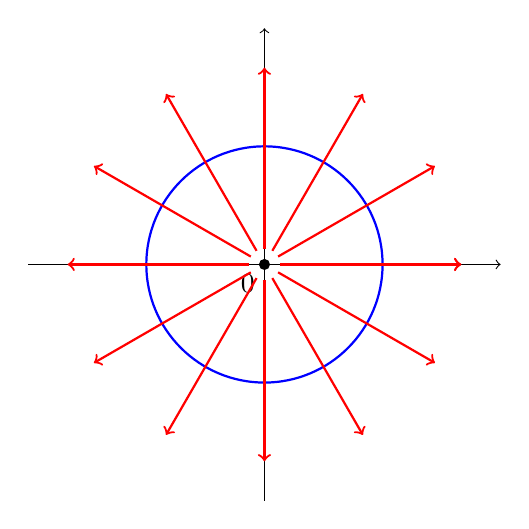
\begin{tikzpicture}
    \draw[->] (-3,0) -- (3,0);
    \draw[->] (0,-3) -- (0,3) node[midway, anchor = north east] {$0$};
    \fill (0,0) circle (2pt);
    \draw[blue, thick] (0,0) circle (1.5);
    \foreach \x in {0,...,12} {
        \draw[red,thick,->] (\x*30:0.2) -- (\x*30:2.5);
    }
\end{tikzpicture}
.\] 
\end{example}

\begin{remark*}
    Der kanonische Isomorphismus ist erstmal $\R^n \setminus \left \{0\right\}  \cong S^{n-1}\times \R$, indem wir $x \mapsto \left( \frac{x}{\lVert x \rVert_2 },\lVert x \rVert _2 \right) $ abbilden. Allerdings ist $\R \cong (0,\infty)$, z.B. mit der Exponentialabbildung.
\end{remark*}


\begin{dexample}[Auf Nachfrage in der Vorlesungspause besprochen]
    Eine Teilmenge $X\subset \R^n$ heißt konvex, wenn für $x,y\in X$ auch die Verbindungsstrecke in $X$ liegt, d.h. für  $λ\in [0,1]$ ist auch $λx + (1-λ)y \in X$. Eine Teilmenge heißt sternförmig, wenn es ein $x_0\in X$ gibt, sodass für jedes $y\in X$ die Verbindungsstrecke von $x_0$ nach $y$ in  $X$ liegt. \\
    Dann sehen wir, dass
    \[
    X \text{ konvex}\implies X \text{ sternförmig} \implies X \text{wegzusammenhängend}
    .\] 
    Die erste Implikation ist trivial, wähle $x_0\in X$ beliebig, für die zweite bilden wir $[0,1]$ einfach auf die Verbindungsstrecke von  $x_0$ nach $y$ ab, dann sind alle Punkte mit  $x_0$ verbunden, und deren Hintereinanderschalten ergibt Wege von $x$ nach  $y$ für  $x,y$ beliebig. \\
    Im Wesentlichen ist das das gleiche Argument, dass wir auch schon für die Intervalle in $\R$ benutzt haben.
\end{dexample}

\section{Lemma von Urysohn}

\begin{theorem}[Urysohn'sches Lemma]\label{thm:urysohn}
    Sei $X$ ein normaler topologischer Raum. Seien  $A,B\subset X$ abegschlossen und disjunkt. Dann existiert eine stetige Abbildung $f: X \to  [0,1]$, sodass $f\mid _A \equiv 0 $ und $f\mid _{B} \equiv  1$.
    \[
\begin{tikzpicture}
    \draw (0,-0.3) -- (4,-0.3) node[anchor=west] {$X$};
    \draw[red,very thick] (0.4,-0.3) -- (1, -0.3) node[midway, anchor = north] {$A$};
    \draw[red, very thick] (2.5,-0.3) -- (3.5, -0.3) node[midway, anchor = north] {$B$};
    \draw[->] (0,0) -- (0,1.5) node[anchor=south] {$\R$};
    \draw (-0.1,0) node[anchor = east] {$0$}-- (0.1,0);
    \draw (-0.1,1) node[anchor=east] {$1$}-- (0.1,1);
    \draw[blue, thick] (0.4,0)-- (1,0);
    \draw[blue, thick] (2.5,1) -- (3.5,1);
    \draw[blue, thick, smooth, domain = 1:2.5,variable=\x] plot ({\x},{(\x-1)^2/2.25});
\end{tikzpicture}
    .\] 
\end{theorem}


\begin{lemma}\label{lm:stetige-abbildung-durch-familie-von-rationalen-offenen-mengen}
    Sei $X$ ein topologischer Raum, sodass für jedes $r\in [0,1]\cap \Q$ offene $V_r \subset X$, sodass $r < r' \implies \overline{V_r} \subset V_{r'}$. Dann existiert eine stetige Abbildung $f: X \to  [0,1]$, sodass $f(x) = 0$ für  $x\in V_0$ und $f(x) = 1$ für  $x\not\in V_1$.
\end{lemma}
\begin{proof}
    Definiere
        \begin{equation*}
        f: \left| \begin{array}{c c l} 
            X & \longrightarrow & [0,1] \\
            x & \longmapsto &  \begin{cases}
                1 & x\not\in V_1 \\
            \inf \left \{r \mid  x\in V_r\right\} & x\not\in V_1
            \end{cases}
        \end{array} \right.
    \end{equation*}
    Die Eigenschaften $f\mid _{V_0} \equiv 0$ und $f\mid _{X \setminus V_i} \equiv  1$ sind sofort klar. Es bleibt zu zeigen, dass $f$ stetig ist. Da
    \[
        \mathcal{S} := \left \{[0,a) \mid  a\in [0,1]\right\}  \cup \left \{(a,1] \mid  a\in [0,1]\right\} 
    .\] 
    eine Subbasis der Topologie auf $[0,1]$ ist, genügt es, Stetigkeit auf  $\mathcal{S}$ zu prüfen. Sei
    \begin{IEEEeqnarray*}{rCl}
        x\in f^{-1}([0,a)) & \iff & f(x) < a \leq  1 \\
                           & \stackrel{\text{Def von $f$}}{\iff} &  \inf \left \{r \mid  x\in V_r\right\} <a \\
                           &\stackrel{\Q \text{ ist dicht}}{\iff} & \exists r < a, r\in \Q \colon x\in V_r \\
                           & \iff&  x\in \bigcup_{r<a} V_r 
    \end{IEEEeqnarray*}
    Für den zweiten Typ von Basielementen ist
    \begin{IEEEeqnarray*}{rCl}
        x\in f^{-1}((a,1]) & \iff& \begin{cases}
                x\not\in V_1 &\text{oder} \\
                x\in V_1, a < f(x) = \inf \left \{r\mid x\in V_r\right\}
        \end{cases} \\
                           & \iff  & \exists r'>a, r'\in \Q, x\not\in V_{r'} \\
                           & \stackrel{\overline{V_r} \subset V_{r'}}{\iff}  & \exists r\in \Q, a<r < r', x\not\in \overline{V_r} \\
                           & \iff  & x\in \bigcup_{r>a} \left( X \setminus \overline{V_r} \right)  
    \end{IEEEeqnarray*}
    also ist auch $f^{-1}((a,1])$ eine Vereinigung von offenen Mengen. \\
    Also ist $f$ stetig, wie zu zeigen war.
\end{proof}

\begin{remark*}
    Wir können uns die $V_r$ wie eine Art 'Höhenprofil' oder 'Höhenlienien' vorstellen, die wir in unserem Raum gegeben haben. 
\end{remark*}

    \lecture[]{Di 18 Mai 2021 12:20}{}
Wir erinnern uns daran, dass wir gerade dabei waren, \autoref{thm:urysohn} zu beweisen.
\begin{lemma}\label{trennung-von-mengen-in-normalem-raum-für-urysohn-lemma}
    Sei $X$ ein normaler Raum,  $A\subset X$ abgeschlossen und $U\subset X$ offen mit  $A\subset U$. Dann existiert $V\subset X$ offen mit
    \[
    A\subset V\subset \overline{V}\subset U
    .\] 
\end{lemma}
\begin{figure}[ht]
    \centering
    \incfig{trennung-von-abgeschlossenen-mengen-durch-offene-in-normalem-raum}
    \caption{trennung von abgeschlossenen mengen durch offene in normalem Raum}
    \label{fig:trennung-von-abgeschlossenen-mengen-durch-offene-in-normalem-raum}
\end{figure}
\begin{proof}
    Wegen $U$ offen ist  $X\setminus U$ abgeschlossen. Wegen $X$ normal gibt es  $V,V'$ offen mit  $A\subset V$ und $(X\setminus U)\subset V'$ mit $V\cap V'=\emptyset$. Nun ist
    \[
    A\subset V\subset X\setminus V' \subset U
    .\] 
    nach Definition des Abschlusses ist nun $A\subset V\subset \overline{V} \subset X\setminus V' \subset U$.
\end{proof}
\todo{bessere abbildung}

\begin{proof}[Beweis von \autoref{thm:urysohn} (\nameref{thm:urysohn})]
    \begin{goal}
        $\forall r\in \Q\cap [0,1]$ konstruiere $V_r \subset X$ offen, sodass
         \begin{enumerate}[1.]
            \item $A\subset V_0$
            \item $B\subset X\setminus V_1$
            \item  $r<r' \implies \overline{V_r}\subset V_{r'}$
        \end{enumerate}
    \end{goal}
Dies genügt, denn dann wissen wir mit \autoref{lm:stetige-abbildung-durch-familie-von-rationalen-offenen-mengen}, dass 
\begin{IEEEeqnarray*}{rCl}
    \exists f: X &\to & [0,1] \text{ stetig} \\
        f(x) & = & 0 \quad \forall x\in V_0 \supset A
        \\ f(x) & = & 1 \quad \forall x \in  X \setminus V_1\supset B
\end{IEEEeqnarray*}
Wähle hierzu eine Abzählung $p_1,p_2,\ldots$ von $\Q\cap [0,1]$, sodass $p_1 = 1$ und $p_2 = 0$. Definiere nun $\left \{V_r\right\} $ rekursiv, wobei wir auch induktiv die Invariante erhalten wollen, dass $r<r' \implies \overline{V_r} \subset V_{r'}$.
\begin{itemize}
    \item $p_1 = 1$. Setze $V_1 \coloneqq X\setminus B$ (offen, weil $B$ abgeschlossen ist)
    \item  $p_2 = 0$. Nach \autoref{trennung-von-mengen-in-normalem-raum-für-urysohn-lemma} mit $A = A$ und  $U = X\setminus B$ finden wir $V_0$ offen mit 
        \[
        A\subset V_0 \subset \overline{V}_0 \subset X\setminus B =: V_1
        .\] 
    \item Sei $n\geq 3$, dann sind also $V_{p_1},V_{p_2},\ldots,V_{p_{n-1}}$ schon definiert. Es ist $\left \{p_1,p_2,\ldots,p_n\right\} $ wohlgeordnet, weil es sich um eine endliche Menge handelt, also gibt es unter ihnen einen direkten Vorgänger $p_i$ von  $p_n$, und einen direkten Nachfolger  $p_j$ von  $p_n$.
         \begin{recap}
            Es könnte z.B.  $n=5$ sein mit \\
            \begin{tabular}{c | c | c | c | c}
                $p_1$ & $p_2$ & $p_3$ & $p_4$ & $p_4$ \\
                1 & 0 & $\frac{1}{2}$ & $\frac{8}{9}$ & $\frac{3}{5}$
            \end{tabular} 
            Dann ist die Menge als $\left \{0,\frac{1}{2},\frac{3}{5},\frac{8}{9},1\right\} $ geordnet, und wir sehen $p_n = $.
        \end{recap}
        Verwende nun \autoref{trennung-von-mengen-in-normalem-raum-für-urysohn-lemma} mit $A = \overline{V_{p_i}}$ und $U = V_{p_j}$, (hier ist wichtig, dass wegen $p_i < p_j$ beretis  $\overline{V_{p_i}}\subset V_{p_j}$ gilt, sonst können wir das Lemma nicht anwenden.) \\
        Also finden wir $V$ mit  $\overline{V_{p_i}} \subset V \subset \overline{V} \subset V_{p_j}$. Man prüft leicht, dass wir so auch die Invariante der Induktion erhalten haben.
\end{itemize}
Also haben wir wie gewünscht die $V_i$ gefunden, und somit unsere Funktion.
\end{proof}

\begin{corollary}[Urysohn mit beliebigem Intervall]\label{cor:urysohn-mit-beliebigem-intervall}
    Sei $X$ ein normaler Raum und seien  $A,B\subset X$ disjunkt und abgeschlossen, sowie $a\leq b\in \R$ beliebig. Dann 
    \begin{IEEEeqnarray*}{rCl}
        \exists f: X & \to  & [a,b] \\
        f(A) & = &\left \{a\right\}  \\
        f(B) & = & \left \{b\right\} 
    \end{IEEEeqnarray*}
\end{corollary}

\begin{proof}
    Verwende einen Homöomorphismus $[0,1] \to  [a,b]$ und \autoref{thm:urysohn}.
\end{proof}
\todo{Beweis ergänzen}

\section{Der Erweiterungssatz von Tietze}
Wir sehen jetzt das \nameref{thm:urysohn} in Action:
\begin{theorem}[Erweiterungssatz von Tietze]\label{thm:thiele}
    Sei $X$ ein normaler Raum und  $A\subset X$ abgeschlossen. Jede stetige Funktion $f: A \to  [-1,1]$ lässt sich fortsetzen zu einer stetigen Funktion $\overline{f}: X \to  [-1,1]$, d.h. $\overline{f}\mid _{A} \equiv f$.
\end{theorem}

\begin{remark}
    Das Urysohn'sche Lemma ist ein Spezialfall des \nameref{thm:thiele}: \\
    Sei $X$ normal und  $B,C\subset X$ abgeschlossen, disjunkt. Dann betrachte die Funktion
        \begin{equation*}
        f: \left| \begin{array}{c c l} 
            B\cup C & \longrightarrow & [-1,1] \\
        B & \longmapsto &  -1 \\
        C & \longmapsto & 1
        \end{array} \right.
    \end{equation*}
    \begin{question}
        Gibt es eine Fortsetzung $\overline{f}: X \to  [-1,1]$?
    \end{question}
    Für jede solche Fortsetzung muss auch  $\overline{f}\mid _{B} = f$, also $\overline{f}(B) = -1$ und $\overline{f}(C) =1$ gelten, also genau das, was wir von Urysohn fordern. \\
    Allerdings sagt uns der \nameref{thm:thiele} genau, dass wir solche eine Fortsetzung finden.
\end{remark}

\begin{proof}[Beweis von \autoref{thm:thiele} (\nameref{thm:thiele}]
    \begin{strategy}
        Wir konstruieren eine Folge stetiger Funktionen \\
        $\left \{s_n : X \to  [-1,1]\right\}_{n\geq 1}$, sodass
        \begin{enumerate}[(i)]
            \item $\left \{s_n\right\} $ konvergiert \vocab{gleichmäßig} gegen eine Funktion $s: X \to  [-1,1]$, d.h. für jedes $ε>0$ existiert  $N\in \N$, sodass 
                \[
                \emphasize{\forall } \in X,n\geq N \colon\qquad    d(s_n(x), s(x))<ε
                .\] 
                Weil $\left \{s_n\right\} $ gleichmäßig konvergiert, ist $s$ stetig (Übungsblatt 5, Aufgabe 3 (iv)).
            \item  $s\mid _{A} = f$
        \end{enumerate}
    \end{strategy}
    Dazu benötigen wir erstmal einige Lemmata, die wir im folgenden erarbeiten.
\end{proof}

\begin{lemma}\label{lm:kompression-von-funktionen-auf-abgeschlossenen-mengen-in-normalem-raum}
    Sei $X$ normal und  $A\subset X$ abgeschlossen. Sei $\alpha : A \to  [-r,r]$ für $r\in \R_{\geq 0}$ stetig. Dann existiert $g: X \to  \left[ -\frac{1}{3}r, \frac{1}{3}r \right]$ stetig mit $\abs{α(a) - g(a)} \leq  \frac{2}{3}r $ für $a\in A$.
\end{lemma}
\begin{proof}
    Setze $B \coloneqq α^{-1}\left(\left[ -r,-\frac{1}{3}r \right]\right)$ und $C\coloneqq α^{-1}\left(\left[ \frac{1}{3}r,r \right]\right)$. Wegen $α$ stetig sind  $B,C$ abgeschlossen, und sie sind auch disjunkt, weil die Intervalle disjunkt sind. Nach \nameref{cor:urysohn-mit-beliebigem-intervall} finden wir also eine stetige Funktion
    \begin{IEEEeqnarray*}{rCl}
        g: X & \to  & \left[ -\frac{1}{3}r, \frac{1}{3}r \right] \\
        g(B) & = & \left \{-\frac{1}{3}r\right\} \\ 
        g(C) & = & \left \{\frac{1}{3}r\right\} 
    \end{IEEEeqnarray*}
    \begin{tikzpicture}
        \draw (0,-0.2) -- (5,-0.2) node[anchor = west] {$X$};
        \draw (0,0) -- (3,0);
        \foreach \x in {0,1,2,3} {
            \draw[red,thin] (0,\x) -- (5,\x);
        }
        \draw (0,0) node[anchor=east] {$-\frac{1}{3}r$};
    \end{tikzpicture}
    \todo{Bild fertig}
    \begin{claim}
        $g$ erfüllt die Bedingungen unseres Lemmas, d.h.  
        \[
        \abs{α(a) - g(a) } \leq \frac{2}{3}r \qquad \forall a\in A
        .\] 
    \end{claim}
    \begin{subproof}
        \begin{itemize}
            \item Sei $a\in B$, Dann ist $α(a) \in \left[ -r, -\frac{1}{3}r \right]$ und $g(a) = -\frac{1}{3}r$, also gilt die Ungleichung.
            \item Sei $a\in C$. Dann ist $α(a) \in \left[ \frac{1}{3}r,r \right]$ und $g(a) = \frac{1}{3}r$, also, also gilt die Ungleichung.
            \item Sei $a\in A \setminus (B\cup C)$. Dann ist $α(a),g(a) \in \left[ -\frac{1}{3}r,\frac{1}{3}r \right] $, und damit ist der Abstand auch höchstens $\frac{2}{3}r$.
        \end{itemize}
    \end{subproof}
\end{proof}
\begin{remark*}
    In der Vorlesung kam die Frage auf, ob wir manche der gerade bewiesenen Resultate auch auf die Analysis übertragen können, indem wir z.B. den Fixpunktsatz von Banach anwenden.
\end{remark*}
\todo{darüber nachdenken}

    % end lectures
    \printindex
    \newpage
    \thispagestyle{plain}
    \printbibliography
    \addcontentsline{toc}{section}{Literatur}
\end{document}
